\section{Simulações}
Para senóides com $f =100 Hz$ e resistores (em Ohms), respectivamente, $R_1 = 100\Omega$, $R_2 = 560\Omega$, $R_3 = 220\Omega$ e $R_4 = 330\Omega$, simule os circuitos A, B e C para todas as combinações de V1, V2 e V3 apresentadas na \textbf{Tabela 1} da \textbf{Folha de Dados}.

\subsection{Circuito A}


\begin{itemize}
    \item Inicialmente, abra o QUCS, vá em \textit{Main Dock} e crie uma nova pasta de projeto. 
    
    \item Na aba Componentes (\textit{Components}), vá em componentes não lineares (\textit{non linar components}) e clique em um Amplificador Operacional (\textit{OpAmp}). Em componentes agrupados (\textit{lumped components}) e clique em dois resistores. Vá em Fontes (\textit{sources}) e coloque uma fonte de tensão AC (\textit{AC voltage Source}).
\end{itemize}

\begin{figure}[H]
    \begin{subfigure}{.4\textwidth}
        \centering
        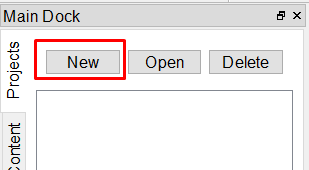
\includegraphics[width=.7\textwidth]{imagens/CircuitoA/new.png}
        \caption{Criação de um novo Projeto}
        \label{fig:new_proj}
    \end{subfigure}    
    \begin{subfigure}{.4\textwidth}
        \centering
        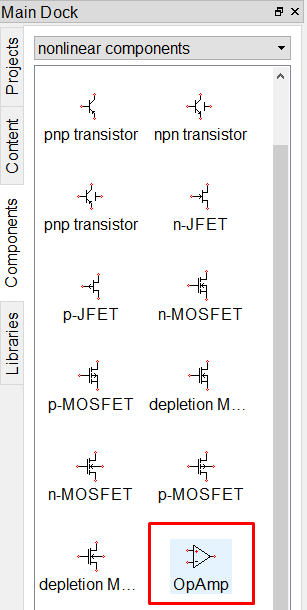
\includegraphics[width=.7\textwidth, trim={ 0 0 0 9cm}, clip]{imagens/CircuitoA/OpAmp.png}
        \caption{Seleção do Amp Op.}
        \label{fig:sel_ampop}
    \end{subfigure}
    
    \begin{subfigure}{.4\textwidth}
        \centering
        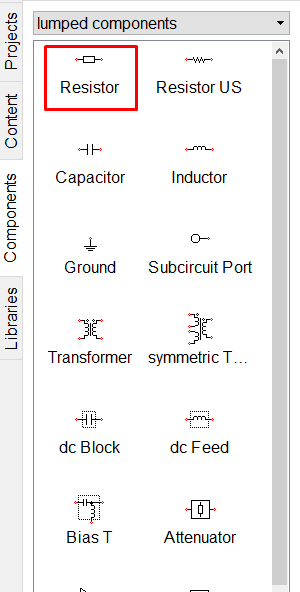
\includegraphics[width=.7\textwidth,  trim={0 7cm 0 0}, clip]{imagens/CircuitoA/resistor.png}
        \caption{Seleção do Resistor.}
        \label{fig:sel_res}
    \end{subfigure}
    \begin{subfigure}{.4\textwidth}
        \centering
        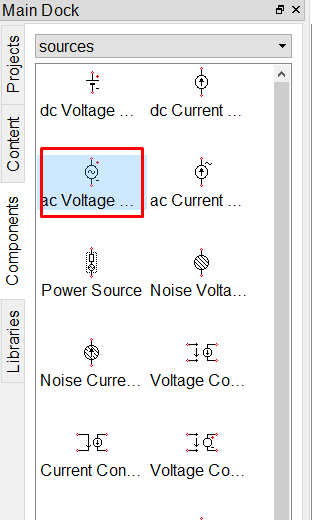
\includegraphics[width=.7\textwidth,  trim={0 7cm 0 0}, clip]{imagens/CircuitoA/fonto_ac.png}
        \caption{Seleção da fonte AC}
        \label{fig:new_proj}
    \end{subfigure}

    \caption{Abertura do projeto e seleção dos componentes }
\end{figure}

\begin{itemize}
    \item Conecte os componentes como a figura \ref{fig:circ_a_q}. Não se esqueça da referência e ajustar os valores dos resistores.
    \item É importante salientar que para essa simulação, necessitaremos de uma simulação AC e outra DC. A simulação AC é necessária para a fonte de voltagem AC, enquanto a fonte DC tem sua utilidade na ligação DC do Amplificador Operacional, \textit{i.e.}, tem seu efeito na energização do $V_{dd}$ e $V_{ss}$ do Amp Op.
    \item  Configure a Simulação AC para observar o valor da saída para a frequência desejada. Salve e simule.
    \item Vá em \textit{Diagramas} e insira uma tabela. Coloque o valor da tensão $V_o.v$. O resultado final deve ser igual ao representado na Figura \ref{fig:circ_a_q}.
    
    \begin{figure}[H]
        \centering
        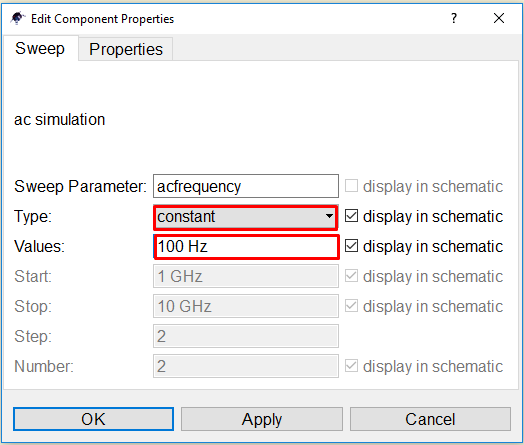
\includegraphics[width=.5\textwidth]{imagens/CircuitoA/simulacao.png}
        \caption{Parâmetros de Simulação AC.}
        \label{fig:my_label}
    \end{figure}
    
\end{itemize}


\begin{figure}[H]
    \centering
    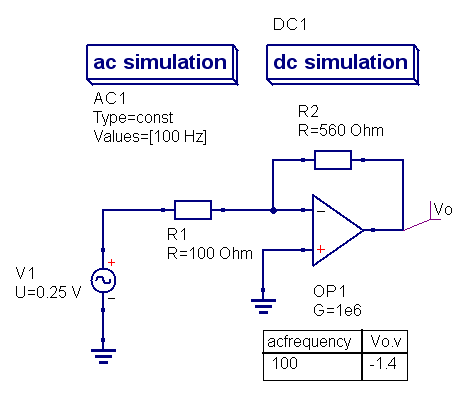
\includegraphics[width=.5\textwidth]{imagens/CircuitoA/circuito_a_sim.png}
    \caption{Arranjo do Circuito A no QUCS.}
    \label{fig:circ_a_q}
\end{figure}

\subsection{Circuito B}
    \begin{itemize}
        \item Vá em arquivo e clique em \textit{Salvar como} e mude o nome do arquivo para utilizar o esquemático já montado para o próximo circuito.
        \item Na aba \textit{Componentes}, vá em componentes agrupados e coloque mais dois resistores. Vá em Fontes e coloque mais duas fontes de tensão AC.
        \item Há duas formas de gerar os circuitos: gerar um por vez, cada qual com seu arquivo; gerar todos de uma só vez, num único arquivo (recomendado).
        \item Nesse tutorial, foi feito todas as variações da tabela 1 da folha de dados em um esquemáticos distintos, como ilustrado nas figuras \ref{fig:2_fon_des}, \ref{fig:1_fon_des} e \ref{fig:0_fon_des}.
    \end{itemize}

\begin{figure}[H]
   
    \begin{subfigure}{.4\textwidth}
        \centering
        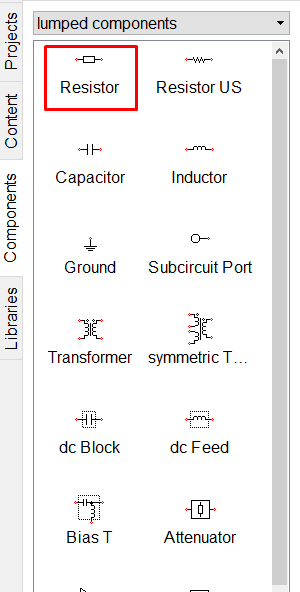
\includegraphics[width=.7\textwidth, trim={0 9cm 0 0}, clip]{imagens/CircuitoA/resistor.png}
        \caption{Seleção dos Resistores}
        \label{fig:sel_resis}
    \end{subfigure}
    \begin{subfigure}{.4\textwidth}
        \centering
        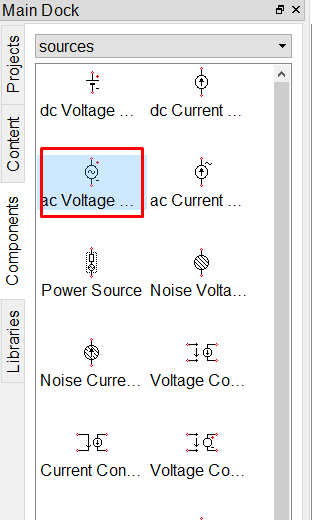
\includegraphics[width=.7\textwidth, trim={0 7cm 0 0}, clip]{imagens/CircuitoA/fonto_ac.png}
        \caption{Seleção fonte AC}
        \label{fig:sel_font_ac}
    \end{subfigure}    
    
 \begin{subfigure}{.45\textwidth}
        \centering
        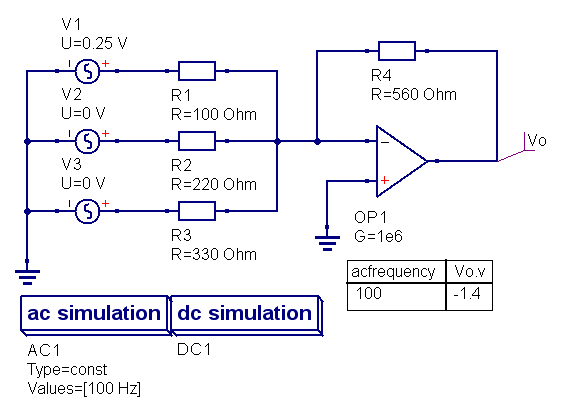
\includegraphics[width=\textwidth]{imagens/CircuitoB/-1_4.png}
        \caption{Uma fonte desativada}
        \label{fig:2_fon_des}
    \end{subfigure}    
    \begin{subfigure}{.45\textwidth}
        \centering
        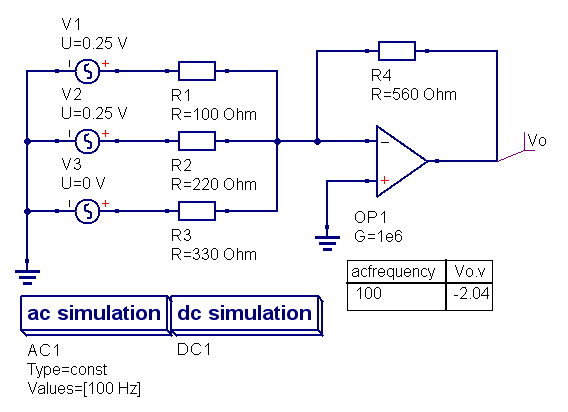
\includegraphics[width=\textwidth]{imagens/CircuitoB/-2_04.png}
        \caption{Apenas uma fonte desativada}
        \label{fig:1_fon_des}
    \end{subfigure}
    \centering
    \begin{subfigure}{.45\textwidth}
        \centering
        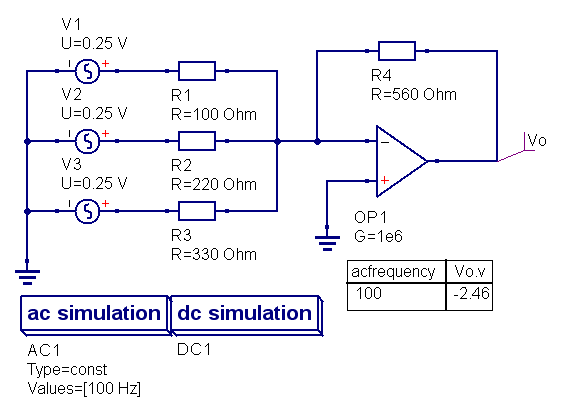
\includegraphics[width=\textwidth]{imagens/CircuitoB/-2_46.png}
        \caption{Todas as fontes Ativas}
        \label{fig:0_fon_des}
     \end{subfigure}
\end{figure}



\subsection{Circuito C}


    \begin{itemize}
        \item Vá em Arquivo e depois em Salvar como... e mude o nome do arquivo para utilizar o esquemático já montado para a o próximo circuito. Exclua a Fonte $V_3$ e conecte os componentes sem esquecer da referência do terra.
        \item Copie  e cole o circuito e modifique os valores das fontes para $V_1 = 0,5V_{pp}$ e $V_2=0V_{pp}$.
        \item Copie e cole em outro espaço, novamente, e modifique os valores das fontes para $V_1 = 0V_{pp}$ e $V_2=0,5V_{pp}$.
        \item Salve e simule.
        \item Vá em Diagramas e insira uma tabela. Coloque o valor das tensões.
        \item Nesse ponto do tutorial, foi colocado todos os circuitos em um único esquemático.
        \item O resultado obtido deve ser semelhante ao apresentado na figura \ref{fig:circuito_c_sim}.
    \end{itemize}

    \begin{figure}[H]
        \centering
        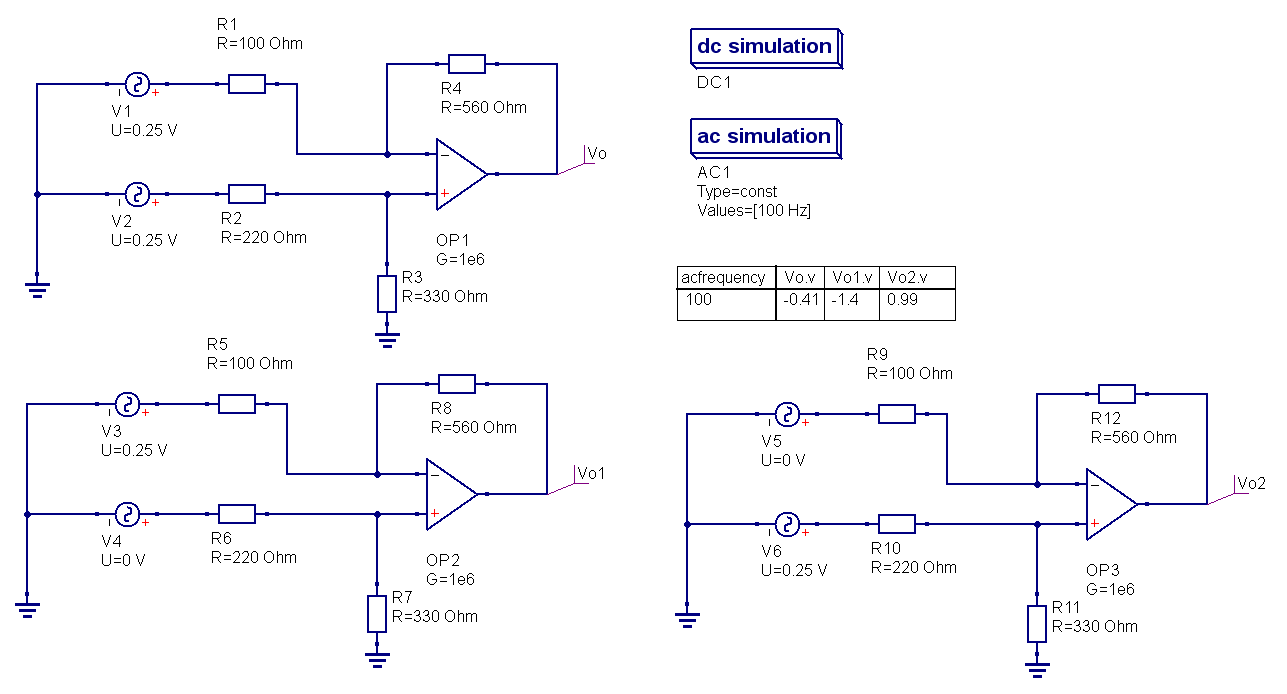
\includegraphics[width=\textwidth]{imagens/CircuitoC/sim_c.png}
        \caption{Esquemático do circuito montado}
        \label{fig:circuito_c_sim}
    \end{figure}